\chapter{Experimental results \status{new}}
\notyetimplemented{}
\todo[inline]{Think about which experiments to do, analyses, comparison with other methods if possible}
	\section{Cell detector \status{new}}
		
	
		Figure \ref{fig:cell_tracks_detection} displays a temporal view of the detected cells. The vertical axis represents the frame of the sequence. The figure clearly shows that ``cell tracks'' are clearly discernible, even if the number of outliers is significant. For the tracking module it is better to have a higher recall than precision, as outliers can be much more easily discarded than segmented tracks linked.
		\begin{figure}
			  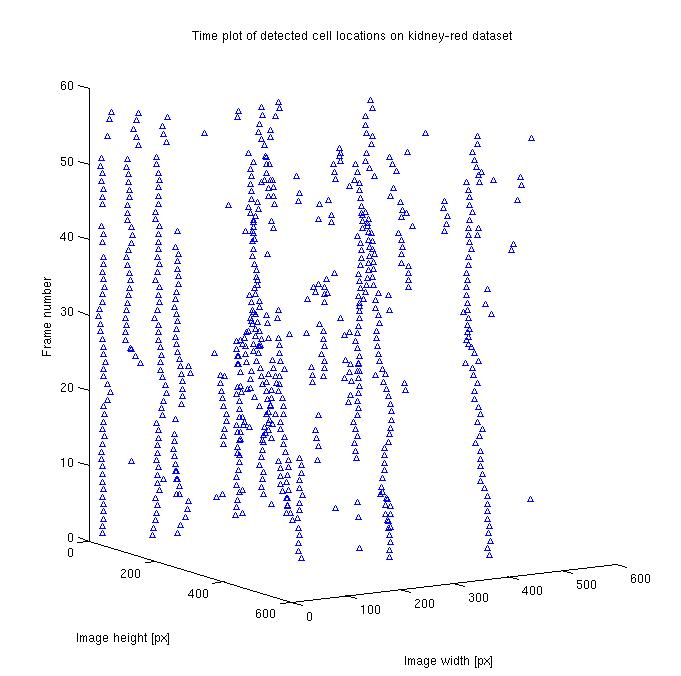
\includegraphics[width=\textwidth]{images/cell_tracks}
			\caption{Cells detected over 60 consecutive frames are visualized as a time series. The vertical axis corresponds to the frames. Even in this raw detection data, it is possible to see the tracks of some of these cells.}
		    \label{fig:cell_tracks_detection}
		\end{figure}
		
			\subsection{Performance \status{new}}
			\todo[inline]{Measure the speed of detection in images of different sizes, and different number of cells}
		
		\subsection{Detection accuracy \status{new}}
	\section{Cell tracker \status{new}}
		\todo[inline]{Define the different measures of accuracy}
		\subsection{Performance metrics \status{new}}
		\subsection{Performance \status{new}}
		\todo[inline]{Meause the speed of generating tracks, as a measure of per 1, 100, 1000 frames, depending on the number of tracks}
		\subsection{Tracking accuracy}